\documentclass{article}

\usepackage{graphicx}
\usepackage{amsmath,amsfonts,amssymb}
\usepackage[colorlinks,bookmarks,bookmarksnumbered,allcolors=blue]{hyperref}
\usepackage[capitalise]{cleveref}
\usepackage[top=0.75in]{geometry}
\usepackage[dvipsnames]{xcolor}
\usepackage{amsmath} 
\usepackage{esvect}

\begin{document}

\author{Joe Spencer}
\title{Leapfrogging Vortex Rings}
\date{}  %August 27, 2022}
\maketitle

\subsubsection*{Methods}
Pairs of vortex rings can move together along a line, appearing to play leapfrog with each other. This phenomenon can occur when the circulation of one vortex ring pulls a second vortex ring forward, and once the second vortex ring has its own inertia moving it forward it begins to pull the first vortex ring. For this assignment, a set of 4 points marking the top and bottom of 2 vortex rings was modeled to leapfrog off of each other, and different graphs and GIFs were created of this behavior. The code used to solve this problem, as well as output data and graphs from the nine drafts of this project, can be found in the LeapFrog branch (\emph{JoeSpencer1-LeapFrog}) of this \href{https://github.com/JoeSpencer1/497R-Projects.git}{GitHub Repository}. \newline

I used the Julia programming language to model these leapfrogging vortices. Julia was especially handy for this project because it could perform calculations on large matrices quickly. Another feature of Julia that became especially handy for this project is its ability to publish figures easily for help visualizing data. Initially, data was written to a file, but recording data to a file was later skipped in the final version to instead dedicate runtime to examining different initial conditions.\newline

Vortices can be described in vector form by Equation 1. This equation shows that the velocity at a point around a vortex is proportional to its circulation, $\vec{\Gamma}$, divided by its distance from the center, $\vec{r}$. $\vec{\Gamma}$ and $\vec{r}$ are crossed to obtain $\vec{V}$, meaning that if $\vec{\Gamma}$ is in the y-direction and $\vec{r}$ is in the x-direction, then the velocity induced by the vortex will be in the y-direction. This also means that an initial velocity is not required for leapfrogging vortices, since the circulation itself will induce that. For my completion of this lab, I used a cross-section of the vortex rings and the x and z-axes with $\vec{\Gamma}$ entirely on the y-axis, pointing into or out of the page.  \newline

\begin{equation} \label{eq:1}
    \begin{aligned}
        \vec{V} &= \frac{\vec{\Gamma} \times \vec{r}}{2 \pi r^2}
    \end{aligned}
\end{equation}

Although $\vec{\Gamma}$ and $\vec{r}$ are crossed, the denominator of Equation 1 contains an r$^2$ term, which means that circulation has a reciprocal relationship with distance, as also expected intuitively. So, in a case where the vortices are further apart, they will be induce less motion in each other. If the vorticity is increased, the vortices will be induced more strongly and move more quickly in their leapfrogging pattern. \newline

This project allowed some freedom to choose initial conditions. In the final version of the project, I have tried 9 different sets of initial conditions. Each vortex was centered around the x-axis. In Table 1, the starting conditions for each set of leapfrogging vortices are listed. This variety of initial conditions yielded a variety of different results, which will be discussed. Table 1 shows the initial position and velocity coordinates and the initial vorticity for each set of leapfrogging vortices. As shown in the table, differences in each of these initial conditions were tested. \newline

\begin{table}
	\centering
	\title{Table 1: Initial Position, Velocity, and Circulation of Each Vortex \newline}
	\title{\emph{A link to a GIF for each vortex is in its far left column.}}
	\begin{tabular}{ | c | c | c | c | c | c | c | c | c |}
		\hline
		GIF & Plot & $f_m$ (Hz) & 1$^{st}$ [$x_0$,$y_0$,$z_0$] & 1$^{st}$ [$\dot{x_0}$,$\dot{y_0}$,$\dot{z_0}$] & $\Gamma_1$ & 2$^{nd}$ [$x_0$,$y_0$,$z_0$] & 2$^{nd}$ [$\dot{x_0}$,$\dot{y_0}$,$\dot{z_0}$] & $\Gamma_2$ \\ \hline
		\href{https://imgur.com/U4cND6X}{1} & \ref{fig:1} & 10 & [1.0,0,1.0] & [0,0,0] & 1.0 & [-1.0,0,1.0] & [0,0,0] & 1.0 \\ \hline
		\href{https://imgur.com/lviamWB}{2} & \ref{fig:2} & 10 & [2.0,0,2.0] & [0,0,0] & 1.0 & [-2.0,0,2.0] & [0,0,0] & 1.0 \\ \hline
		\href{https://imgur.com/6jT1mT0}{3} & \ref{fig:3} & 100 & [1.0,0,1.0] & [0,0,0] & 1.0 & [-1.0,0,1.0] & [0,0,0] & 1.0 \\ \hline
		\href{https://imgur.com/PtazOFB}{4} & \ref{fig:4} & 1 & [1.0,0,1.0] & [0,0,0] & 1.0 & [-1.0,0,1.0] & [0,0,0] & 1.0 \\ \hline	
		\href{https://imgur.com/wSpWEQV}{5} & \ref{fig:5} & 10 & [1.0,0,1.0] & [0,0,0] & 1.0 & [-1.0,0,1.0] & [0,0,0] & -1.0 \\ \hline
		\href{https://imgur.com/aZzMnJV}{6} & \ref{fig:6} & 10 & [1.0,0,1.0] & [0,0,0] & 2.0 & [-1.0,0,1.0] & [0,0,0] & 1.0 \\ \hline
		\href{https://imgur.com/nKVGuJ9}{7} & \ref{fig:7} & 10 & [0.75,0,0.75] & [0.2,0,0] & 2.5 & [-0.8,0,0.6] & [0,0,0] & 2.5 \\ \hline
		\href{https://imgur.com/UZyBsYO}{8} & \ref{fig:8} & 10 & [1.0,0,1.0] & [0.006,0,0.008] & 1.0 & [-1.0,0,1.0] & [0,0,0] & 1.0 \\ \hline
		\href{https://imgur.com/tctJPyS}{9} & \ref{fig:9} & 10 & [1.0,0,1.0] & [0.2,0,0.1] & 3.0 & [-1.0,0,1.0] & [0.2,0,0.1] & 3.0 \\ \hline
	\end{tabular}
\end{table}

The final program for modeling leapfrogging vortices also allowed the user to adjust the number of steps the program would simulate and the length of each time step, but these parameters were left at 0.1 seconds and 1,000 steps for most of the program. Shorter and longer time steps between measurements were tried, but the lower frequency shown in \href{https://imgur.com/PtazOFB}{GIF 8} diverged from the actual solution for the leapfrogging vortices, and the higher calculation frequency modeled in \href{https://imgur.com/6jT1mT0}{GIF 9} only slowed down the program while measuring fewer vortices that were not substantially different. \newline

Once I understood that I was to model the top and bottom points of 2 vortices, it was relatively smooth sailing to establish a working code. To make this model I used the DeliniatedFiles, Printf, and Plots libraries in Julia. After I had created a good model, I decided to animate it. I eventually found that to be fairly simple. I used the \textcolor{Dandelion}{@animate} function to make a gif for each vortex. These can be viewed either by clicking the colored number links in the table, or by going to the LeapFrog branch of the \href{https://github.com/JoeSpencer1/497R-Projects.git}{GitHub Repository} mentioned previously. \newline

\subsubsection*{Results and Discussion}

This lab examined how vortices can perpetuate each other. The following nine figures show the different paths followed by each vortex pair in this experiment. The results shown in these graphs provide insights about when the phenomenon of vortex leapfrogging occurs, and when it does not.\newline

This experiment found that vortices that have either both positive or both negative circulation directions can leapfrog off each other. If they have the same circulation, they can go on a very long time in a low resistance environment, as seen in Figure \ref{fig:1} and Figure \ref{fig:2}. In a real environment, energy would be required to continue the vortex rings along their same trajectories, but the vortex rings in Figure \ref{fig:1}, Figure \ref{fig:2}, and \ref{fig:3} each experienced no change in their patterns between cycles. \newline

Two figures, Figure \ref{fig:3} and Figure \ref{fig:4}, were recorded to test different sample frequencies. Both the sample frequencies 10 times slower and 10 times faster were deemed inappropriate or unnecessary. The slower sample frequency did not pick up changes in the velocity of particles and provided an inaccurate solution. The faster sampling frequency obtained the same results as the 10 Hz frequency used for this simulation, but took 10 times as long to obtain data for the same simulations. These frequencies would likely need to be refined, though, for simulations of significantly stronger, weaker larger. or smaller vortex rings. \newline

If the circulations have opposite directions, as in Figure \ref{fig:5}, they repel each other instead of leapfrogging. This experiment also discovered that if the vortices have different circulations, then their leapfrogging patterns will change as they move away from each other. An examples of this can be seen in Figure \ref{fig:6}. Although it this pair of vortex rings appears to be traveling in a pattern, the tops and bottoms of the second cycle are further apart. Figure \ref{fig:7} shows what occurs when have very different initial velocities. The vortices also leapfrog some in this case, but eventually separate.\newline

Figure \ref{fig:8} and Figure \ref{fig:9} show another interesting property of leapfrogging vortex ring pairs. The vortex pairs represented by these two figures travel in a direction that is not totally orthogonal to both their alignment and vorticity. The vortex rings in Figure \ref{fig:8} travel in different directions and separate and even break very quickly. The vortex rings in Figure \ref{fig:9}, on the other hand, travel in the same direction. Their paths can still be seen changing in shape and diverging, though, albeit slightly more slowly. \newline

One interesting relationship to note in the vortex rings that this experiment found is that for vortex rings that go on the longest, the velocity is inversely proportional to the distance. This can be recalled from Equation \ref{eq:1}, which showed that the magnitude of velocity is directly proportional to circulation and ultimately inversely proportional to distance. The 
\href{https://imgur.com/U4cND6X,}{videos} included in this report show that show that for the vortices that continued longest, the highest velocity occurred when \emph{r} was smallest, and lowest velocity came when \emph{r} between the top and bottom vortices of the ring was greatest. \newline

\begin{figure}[htb]
	\centering
	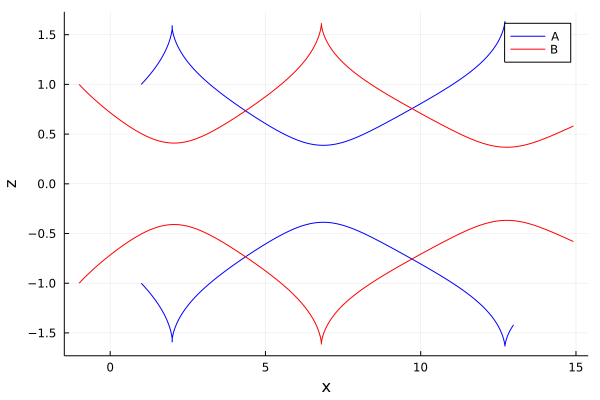
\includegraphics[width=\textwidth]{Graph_A.png}
	\caption{Paths of First Pair Leapfrogging Vortex Rings\newline This figure shows two vortex rings leapfrogging in the expected fashion.}
	\label{fig:1}
\end{figure} 

\begin{figure}[htb]
	\centering
	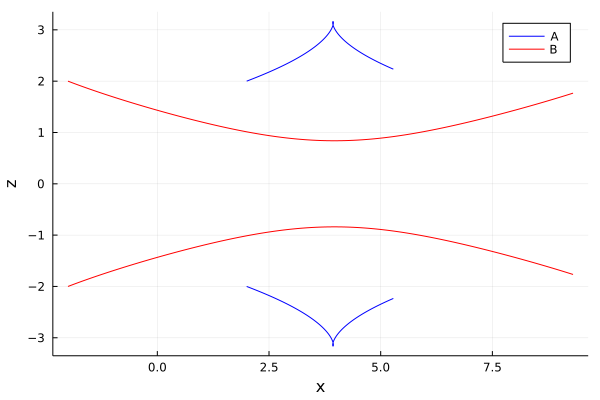
\includegraphics[width=\textwidth]{Graph_D.png}
	\caption{Second Pair of Leapfrogging Vortex Rings\newline The distance between the vortex rings is doubled in Figure 2.}
	\label{fig:2}
\end{figure} 

\begin{figure}[htb]
	\centering
	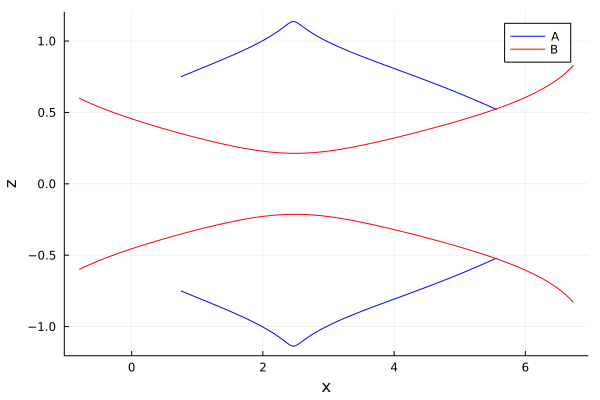
\includegraphics[width=\textwidth]{Graph_I.png}
	\caption{Third Pair of Leapfrogging Vortex Rings\newline Measurements in Figure 3 were taken ten times as often. It war hard to get much data.}
	\label{fig:3}
\end{figure} 

\begin{figure}[htb]
	\centering
	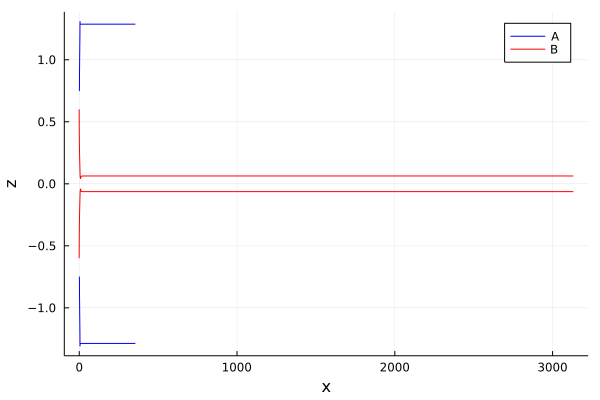
\includegraphics[width=\textwidth]{Graph_H.png}
	\caption{Fourth Pair of Leapfrogging Vortex Rings\newline This figure shows that a one-second measurement interval is too long.}
	\label{fig:4}
\end{figure} 

\begin{figure}[htb]
	\centering
	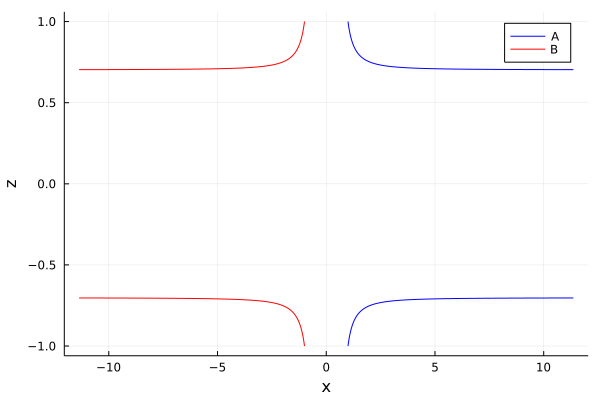
\includegraphics[width=\textwidth]{Graph_B.png}
	\caption{Fifth Pair of Leapfrogging Vortex Rings\newline This separation instead of leapfrogging happens when the rings have strength $\Gamma$ in oppostie directions.}
	\label{fig:5}
\end{figure} 

\begin{figure}[htb]
	\centering
	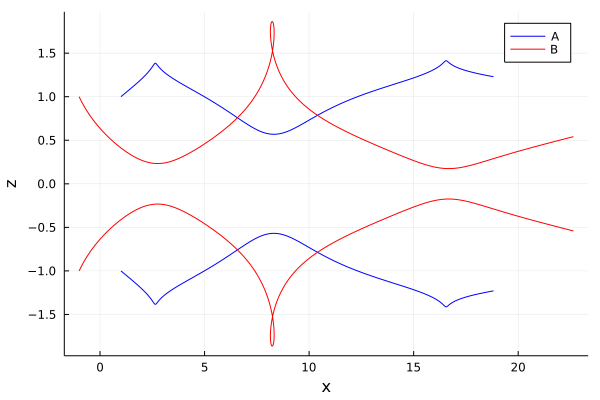
\includegraphics[width=\textwidth]{Graph_C.png}
	\caption{Sixth Pair of Leapfrogging Vortex Rings\newline In Figure 6, one vortex ring has a circulation twice as high as the other.}
	\label{fig:6}
\end{figure} 

\begin{figure}[htb]
	\centering
	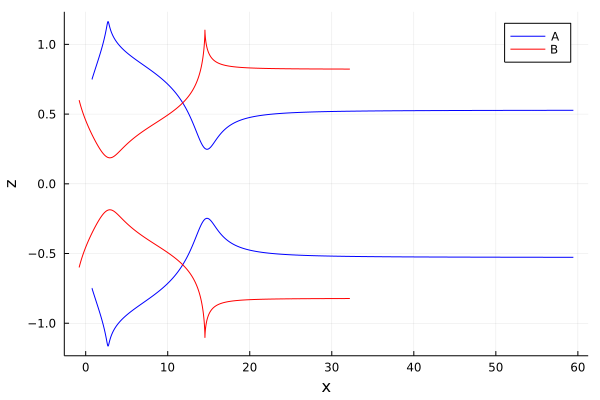
\includegraphics[width=\textwidth]{Graph_G.png}
	\caption{Seventh Pair of Leapfrogging Vortex Rings\newline In Figure 7, one vortex ring travels more quickly than the other and quickly leaves it behind.}
	\label{fig:7}
\end{figure} 

\begin{figure}[htb]
	\centering
	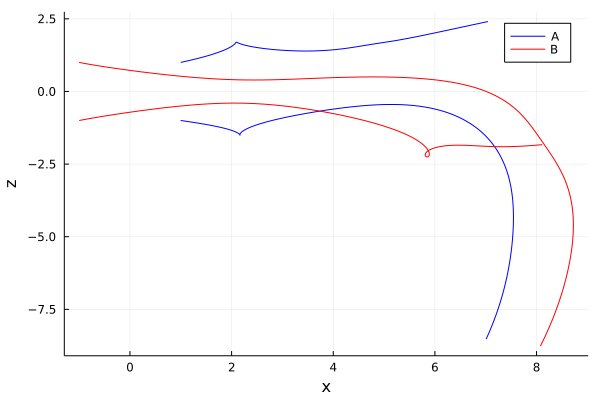
\includegraphics[width=\textwidth]{Graph_E.png}
	\caption{Eighth Pair of Leapfrogging Vortex Rings\newline One vortex in the eighth pair of leapfrogging vortex rings started out with an initial velocity in the x-direction and an initial velocity in the y-direction.}
	\label{fig:8}
\end{figure} 

\begin{figure}[htb]
	\centering
	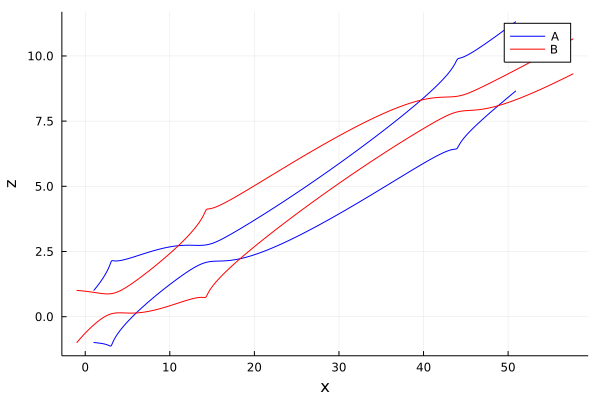
\includegraphics[width=\textwidth]{Graph_F.png}
	\caption{Ninth Pair of Leapfrogging Vortex Rings\newline Figure 9 shows how vortex rings traveling in slightly different directions diverge.}
	\label{fig:9}
\end{figure} 

\end{document}